% !TeX root = ../main.tex
% Add the above to each chapter to make compiling the PDF easier in some editors.

\chapter{Introduction}\label{chapter:introduction}
The rapid and continuous development of \ac{AI} has given birth to numerous
applications that have pushed the boundaries of what we previously believed to be possible.
This thesis will delve into one of the most fascinating and alarming developments in this
field, deepfakes. This work aims to help readers in understanding how deepfakes are
identified, along with their current limitations, and potential future research directions.



\section{Background and Motivation}\label{chapter:backgroundAndMotivation}
In an era where digital media forms the cornerstone of communication, the advent of deepfakes,
\ac{AI}-enabled synthetic media, poses an unprecedented challenge to information integrity.
Deepfakes, a portmanteau of `deep learning' and `fake'~\cite{Gardiner2019FacialRS,10.1145/3425780,Nguyen_2022},
is a technology that manipulates or fabricates audio-visual content to make it appear
real, often indistinguishable from the original~\cite{10.1145/3543873.3587581}. An example of a generated and altered image can be seen in~\autoref{fig:bill-hader}
\begin{figure}[hb]
	\centering
	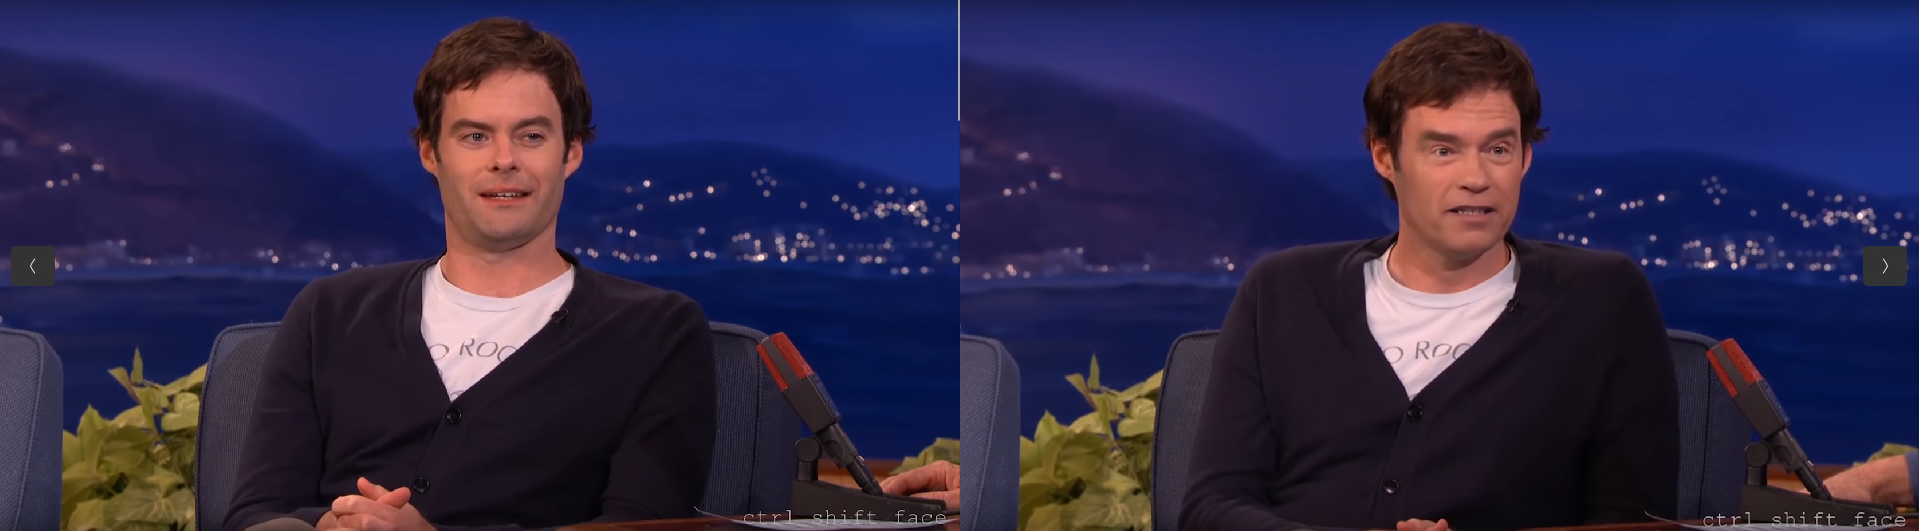
\includegraphics[scale=0.289]{figures/bill-arnold}
	\caption{Deepfake of Bill Hader impersonating Arnold Schwarzenegger. Screenshot from~\cite{bill-hader}}\label{fig:bill-hader}
\end{figure}

The proliferation of deepfake technology become initially sparked with the aid of
its software in creating misleading movie star images and videos, before quickly
expanding into different sectors. One of the earliest examples that drew widespread
interest to deepfakes was a video made by an anonymous Reddit user named `deepfakes'
in late 2017~\cite{10.1145/3491102.3517446, 10.1145/3425780}.
This consumer started to publish digitally altered pornographic motion pictures,
realistically swapping the faces of actresses onto the bodies of porn stars.
While these explicit videos were quickly removed, the sudden emergence of this facial
replacement method, quickly caught the media's eye and circulated on various online forums~\cite{albahar2019deepfakes}.
However, it didn't take long for the technology to be applied beyond explicit content.

A notable example that showcased the potential of deepfakes,
and arguably delivered it to mainstream attention, turned into a video of former
U.S. President Barack Obama, released in April 2018 by Buzzfeed and Jordan Peele~\cite{peele,10.1145/3371409}.
The video features a deepfake of Obama announcing matters he by no means clearly
stated, with Peele providing the voiceover. This deepfake video effectively highlighted
the potential misuse of this technology in spreading misinformation and propaganda.

In recent years, the sophistication of deepfake technology has reached an unprecedented level.
An interesting example of this progression can be seen in the creation of `Tom Cruise deepfakes'
that circulated on social media in early 2021~\cite{deeptomcruise-article}. The videos, created by Belgian visual effects
artist Chris Ume in collaboration with actor Miles Fisher, who impersonated Cruise's voice
and mannerisms, were shared on TikTok under the account name
@deeptomcruise\footnote{\url{https://www.tiktok.com/@deeptomcruise}}~\cite{Agarwal_2021_CVPR,belive-or-not}.
These deepfake videos show the synthetic `Tom Cruise' doing various activities --- performing
a magic trick, playing golf, or simply telling a story about Mikhail Gorbachev~\cite{deeptomcruise}.

The `Tom Cruise deepfakes' took the internet by storm due to their uncanny resemblance to the
real actor, in terms of both appearance and behavior. Unlike the early deepfake videos, which
often exhibited glaring imperfections, these deepfakes were so convincing that many viewers
initially believed they were watching the actual Tom Cruise. This level of realism underscored
the strides made in deepfake technology, while simultaneously highlighting the potential
dangers of its misuse.

Driven by advances in machine learning, especially deep learning, deepfake technology has
grown significantly in sophistication and accessibility. The potential applications of
deepfakes range from benign, such as in film production and entertainment, to malicious uses,
including disinformation campaigns, identity theft, and deepfake pornography. As these
applications become more widespread, deepfake technology has raised profound questions and
challenges for society, especially regarding media authenticity, privacy, and cybersecurity.

However, it is not just the creation of deepfakes that has improved; strides have also been made
in detection. There are now more sophisticated, \ac{AI}-powered tools that can analyze videos
and images for signs of manipulation. These tools operate on multiple levels, from detecting
inconsistencies in lighting and shadows to looking for signs of digital artifacts and abnormal
facial movements. But as detection tools become more sophisticated, so too do the techniques
used to create deepfakes. This constantly evolving technological arms race underscores the
critical need for ongoing research and development in deepfake detection.

In response to these challenges, there is an increasing need for robust and reliable
deepfake detection tools. However, despite the flurry of research and development in this
area, a comprehensive understanding and evaluation of the available detection tools remain
elusive. This knowledge gap not only impedes the technological advancements in deepfake
detection but also complicates the task of policy-making and regulation in this sphere.

This thesis is motivated by the need to bridge this gap and advance our understanding of
publicly-available deepfake detection tools. By examining these tools, this study aims to
contribute to the ongoing efforts to mitigate the risks associated with deepfakes and uphold
the integrity of digital media.


\section{Thesis Structure}\label{chapter:structure}
Understanding the structure of this thesis is essential for a thorough understanding of the
research, as it follows a logical and systematic progression. It starts by laying the basic
groundwork, then gradually delves deeper into the specifics of the study, eventually
integrating the findings and projecting forward-looking discussions. Below is a
detailed outline of the thesis structure, which serves as a roadmap for navigating
the document.

This initial chapter lays the foundation for the thesis. It provides an overview of deepfakes,
introduces the topic of deepfake detection, and outlines the significance and timeliness
of the study. It presents the objectives of the research by addressing three research
questions, clearly stating what the study aims to achieve. The scope and limitations are
also discussed here, delineating the boundaries of the research and acknowledging
its constraints. The introduction serves as a guide, setting the reader's expectations
for the rest of the thesis.

The literature review provides a survey of the existing body of knowledge
related to deepfakes and their detection. The section begins with an explanation of the
techniques used to create deepfakes, giving the reader an understanding of the
technology behind them. This section also highlights the ethical and legal concerns
surrounding deepfakes and the countermeasures and detection methods currently in place.
By identifying gaps and shortcomings in the existing literature, this section also
underscores the relevance and value of the present study.

Chapter three, the methodology along with evaluation metrics and datasets
adopted for the study are outlined. The chapter provides information on how
the publicly-available deepfake detection tools were selected for analysis.
It also discusses the evaluation metrics used to test the effectiveness of these
tools and the datasets used for testing. By detailing these elements, the chapter
ensures that the research process is transparent and replicable.

Chapter four offers an analysis of the six deepfake detection tools: three for video
and three for images. These tools were tested using metrics from~\autoref{chapter:methodology},
looking at their functionality, advantages, and drawbacks.

The fifth chapter takes the analysis from theory to practice, exploring real-world instances
where deepfakes and their detection have played a significant role. The case studies
are chosen to represent a variety of scenarios, thereby providing some of the
practical implications and challenges associated with deepfakes and their
detection.

The sixth chapter presents the findings from the evaluation of the selected tools.
It also provides a comparative analysis of the tools, highlighting their relative
strengths and weaknesses. Subsequently, the results of the comparison are described
and discussed. The research questions from~\autoref{sec:objectives} are also answered here.

The final chapter summarizes the findings and discussions from previous chapters and
reflects on their contribution to the field. It also identifies potential directions
for future research, offering suggestions for how the field can continue to evolve
and adapt in response to the dynamic nature of deepfakes. Finally, a conclusion is drawn,
highlighting current deepfake limitations.

\section{Objectives of the Study}\label{sec:objectives}
Deepfakes have been prominently discussed in both scholarly articles and the media~\cite{forbes-2020,guardian-2019}.
Their ability to convincingly deceive an ordinary user is getting better and better.
For effective countermeasures and understanding of future threats, it's important to understand
deepfake detection technologies. Thus, the primary purpose of the thesis is to provide
an exploration of the state of the art in publicly-available deepfake detection tools.
Specifically, the study addresses these \ac{RQ}:

\begin{itemize}
	\item Research Question 1: How accessible and user-friendly are publicly-available
	      deepfake detection tools for individuals who do not have expertise in deepfakes or
	      detectin deepfakes?
	\item Research Question 2: How effective are deefake detection tools, which are selected
	      and analyzed in this research, in identifying forgeries from various deepfake
	      generation tools?
	\item Research Question 3: What are the privacy implications and policies associated with
	      selected deepfake detection tools?
\end{itemize}

To address the first research question, a methodological approach was adopted. The selection
criteria, encompassing factors like accessibility, user-friendliness, and documentation
are explained. These criteria guide the selection of the six tools examined in this study.
Subsequently, the evaluation metrics are established to assess the strengths and shortcomings
of these detection tools. Initially, all tools undergo an evaluation based on the selection
criteria outlined in~\autoref{chapter:methodology}. The assessment considers factors like
the tool's accessibility, and determining if it's open-source or proprietary. The availability
of support and documentation, including installation guides and usage instructions, is also
examined. The presence or absence of source code, difficulty of use, any internet or
specific software and hardware requirements, and whether the tools are free or paid,
are also considered. These evaluations are detailed further in~\autoref{sec:analysis-tools}.

In response to the second research question, the study evaluates the performance of the
selected tools against a range of deepfakes generated through diverse methods. Initially,
each of the six tools undergoes testing to discern if they can detect deepfakes. The video
detection tools are evaluated using 110 videos, comprising 40 deepfake videos from
DeepFaceLab~\cite{perov2021deepfacelab}, 40 from FaceSwap~\cite{faceswap}, 10 deepfake
videos sourced from the FaceForensics++~\cite{roessler2019faceforensicspp} dataset,
and 20 authentic videos from the same dataset. Image detection tools are assessed using a
total of 123 images: 49 deepfakes produced with FaceApp~\cite{faceapp-app},
54 with Stable Diffusion~\cite{stable-diffusion}, and 20 genuine photographs obtained online.
Furthermore, the training models and techniques utilized, the datasets employed for initial tool
testing, and the programming languages and frameworks are also examined to answer this question.

Regarding the third research question, attention is directed towards the privacy measures of the
selected tools, examining the presence of their privacy policies and their user data handling
methods. This involves examining the potential risks and determining if the tool developers
provide Terms of Use and Privacy Policy for their tools' utilization.

The identification and elaboration of these research questions provide a roadmap for the study,
with each one serving as a crucial stepping-stone toward the understanding of the nature of
the selected publicly-available detection tools. The research questions are then answered in~\autoref{chapter:results},
comparing the strengths and limitations of the selected tools.

\section{Scope and Limitations}\label{chapter:scope}
The study of deepfakes and their detection is a broad field, involving a range of complex and
interrelated topics. Therefore, it is essential to define the specific scope and
limitations of this thesis to clarify what it will and will not cover. These boundaries
not only provide clarity but also help ensure that the research is feasible and can delve
into the chosen topics in sufficient depth.

\subsection{Scope of the Study}
The primary focus of this thesis is on the analysis and evaluation of publicly available
deepfake detection tools. It will cover both the technical and societal aspects of these
tools, including their performance, methodologies, implications, and potential areas for
future development. It will also provide an overview of the current state of deepfake
technology, from its historical development to its modern techniques and applications.

The thesis will mainly concentrate on visual deepfakes, encompassing both images and
videos, aiming to offer an understanding of the deepfake environment. The
research will also explore the dual nature of deepfakes, examining their harmless
and harmful applications. This exploration is crucial to understand the
difficulties involved in detecting deepfakes.

\subsection{Limitations of the Study}
Despite its broad scope, the study is subject to several limitations that should be
acknowledged. Firstly, due to the rapid pace of technological advancements in the field
of deep learning and \ac{AI}, the state of the art in deepfake technology and detection tools
can change swiftly. As a result, while the thesis aims to provide an up-to-date overview
of the field, some of the information might become outdated shortly after publication.

Secondly, given the focus on publicly-available tools, this thesis might not capture
the full spectrum of deepfake detection methodologies. Many sophisticated tools and
techniques might be proprietary or classified information, not accessible for public
use or scrutiny. Thus, while this study will provide an overview of the
available tools, it might not cover the absolute cutting edge in deepfake detection.

Thirdly, while the study aims to objectively evaluate the performance of deepfake
detection tools, it's important to note that this evaluation is based on the
available datasets and metrics. Variations in these datasets, such as the quality
and diversity of the deepfakes included, can impact the results. Moreover, no
single evaluation metric or dataset can fully capture the effectiveness of a tool
in all real-world scenarios.

Fourthly, while the study will explore the societal, ethical, and legal implications
of deepfakes and their detection, a full analysis of these complex and
evolving issues is beyond its scope. These aspects will be discussed primarily in
relation to the main focus of the thesis --- deepfake detection tools --- and may not
cover all the potential implications of deepfakes.

Finally, the study is limited by the inherent challenges associated with deepfake
detection. Deepfakes are a result of advanced \ac{AI} and machine learning techniques,
and detecting them is a complex task that is still an area of active research.
Therefore, the study's findings should be viewed in light of these inherent difficulties.

\subsection{Delimitations of the Study}
While limitations are factors that are out of the researcher's control, delimitations
are boundaries set by the researcher. In this study, due to time and resource constraints,
the analysis will be limited to a few publicly-available deepfake detection tools,
rather than a list of all available tools. Similarly, while the study will discuss
a few illustrative examples of deepfake applications and case
studies, it will not provide a comprehensive review of all possible uses or instances
of deepfakes.

By acknowledging these scope, limitations, and delimitations, this thesis aims to
provide a clear exploration of publicly-available deepfake detection tools while
being transparent about its boundaries and potential areas of uncertainty.
